\documentclass[a4paper,11pt]{article}
\usepackage{amsmath,amsthm,amsfonts,amssymb,amscd,amstext,vmargin,graphics,graphicx,tabularx,multicol} 
\usepackage[francais]{babel}
\usepackage[utf8]{inputenc}  
\usepackage[T1]{fontenc} 
\usepackage{pstricks-add,tikz,tkz-tab,variations}
\usepackage[autolanguage,np]{numprint} 
\usepackage{calc}

\setmarginsrb{1.5cm}{0.5cm}{1cm}{0.5cm}{0cm}{0cm}{0cm}{0cm} %Gauche, haut, droite, haut
\newcounter{numexo}
\newcommand{\exo}[1]{\stepcounter{numexo}\noindent{\bf Exercice~\thenumexo} : }
\reversemarginpar

\newcommand{\bmul}[1]{\begin{multicols}{#1}}
\newcommand{\emul}{\end{multicols}}

\newcounter{enumtabi}
\newcounter{enumtaba}
\newcommand{\q}{\stepcounter{enumtabi} \theenumtabi.  }
\newcommand{\qa}{\stepcounter{enumtaba} (\alph{enumtaba}) }
\newcommand{\initq}{\setcounter{enumtabi}{0}}
\newcommand{\initqa}{\setcounter{enumtaba}{0}}

\newcommand{\be}{\begin{enumerate}}
\newcommand{\ee}{\end{enumerate}}
\newcommand{\bi}{\begin{itemize}}
\newcommand{\ei}{\end{itemize}}
\newcommand{\bp}{\begin{pspicture*}}
\newcommand{\ep}{\end{pspicture*}}
\newcommand{\bt}{\begin{tabular}}
\newcommand{\et}{\end{tabular}}
\renewcommand{\tabularxcolumn}[1]{>{\centering}m{#1}} %(colonne m{} centrée, au lieu de p par défault) 
\newcommand{\tnl}{\tabularnewline}

\newcommand{\trait}{\noindent \rule{\linewidth}{0.2mm}}
\newcommand{\hs}[1]{\hspace{#1}}
\newcommand{\vs}[1]{\vspace{#1}}

\newcommand{\N}{\mathbb{N}}
\newcommand{\Z}{\mathbb{Z}}
\newcommand{\R}{\mathbb{R}}
\newcommand{\C}{\mathbb{C}}
\newcommand{\Dcal}{\mathcal{D}}
\newcommand{\Ccal}{\mathcal{C}}
\newcommand{\mc}{\mathcal}

\newcommand{\vect}[1]{\overrightarrow{#1}}
\newcommand{\ds}{\displaystyle}
\newcommand{\eq}{\quad \Leftrightarrow \quad}
\newcommand{\vecti}{\vec{\imath}}
\newcommand{\vectj}{\vec{\jmath}}
\newcommand{\Oij}{(O;\vec{\imath}, \vec{\jmath})}
\newcommand{\OIJ}{(O;I,J)}


\newcommand{\reponse}[1][1]{%
\multido{}{#1}{\makebox[\linewidth]{\rule[0pt]{0pt}{20pt}\dotfill}
}}

\newcommand{\titre}[5] 
% #1: titre #2: haut gauche #3: bas gauche #4: haut droite #5: bas droite
{
\noindent #2 \hfill #4 \\
#3 \hfill #5

\vspace{-1.6cm}

\begin{center}\rule{6cm}{0.5mm}\end{center}
\vspace{0.2cm}
\begin{center}{\large{\textbf{#1}}}\end{center}
\begin{center}\rule{6cm}{0.5mm}\end{center}
}



\begin{document}
\pagestyle{empty}
\titre{Séance d'AP . . . : Notions de vitesse}{}{}{4ème}{}

\vspace*{0.2cm}


\exo \\
Application des formules\\

\noindent \q Un piéton met 2h pour parcourir 12,8 km. Quelle est sa vitesse moyenne en km/h ?\\
\q Un camion roule pendant 3h à une vitesse moyenne de 85 km/h. Quelle est sa distance parcourue en km ?\\
\q Une voiture roule à une vitesse moyenne de 75,5 km/h et parcourt 181,2 km. Quelle est la durée du parcours  en heures et minutes ?\\




\exo \\Supposons que la longueur de la pente du volcan vaut 2 610 m et que la nuée ardente dévale cette pente à une vitesse de 4,58 km/min.\\

\noindent \initq 
\q Transformer la vitesse en m/s puis en km/h.\\
\q Combien de temps la nuée ardente va t-elle mettre pour dévaler la pente ?\\

\begin{center}
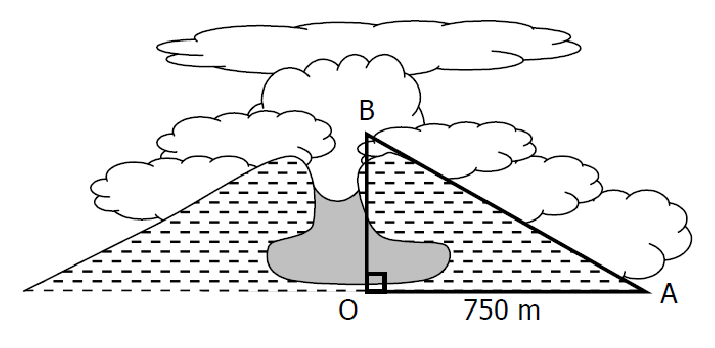
\includegraphics[scale=0.9]{vitesse1.eps} 
\end{center}

\vspace*{0.3cm}


\exo \\
Nina est aux Estables pour une « sortie-ski » avec sa classe. Elle est au pied du TELESKI CHALET 2 où personne n'attend. Il est 16 h 50 et son professeur a donné rendez-vous au pied des pistes à 17 h précises pour le retour. \\
Nina descend en moyenne à 15 km/h. \\
\textbf{A-t-elle le temps de faire une dernière descente si elle emprunte une de ces 2 pistes ?}(Justifier votre réponse)\\

\textit{Dans cette question, toute trace de recherche, même incomplète, ou d'initiatives, même
infructueuses, sera prise en compte dans l'évaluation.}\\

\begin{center}
\includegraphics[scale=0.65]{vitesse3.eps}  \includegraphics[scale=0.65]{vitesse3b.eps}  
\end{center}





\end{document}
